%-------------------------------------------------------------------------------
%                                PREAMBLE
%-------------------------------------------------------------------------------
\documentclass[usenames,dvipsnames,svgnames,10pt,aspectratio=169]{beamer}
%
\usefonttheme{professionalfonts}
% This theme uses TIKZ: compile twice with PDFLaTeX or LuaLaTeX.
%
%  Options:
%  - [clean]:    clean slides, i.e. logos and footbar are removed
%  - [kth]:      footbar style inspierd to the official KTH template
%  - [nicewave]: a different style of wave is used (not approved by FLOW)
%
\usetheme[clean]{flow}

\usepackage{tikz}
\usetikzlibrary{arrows}
\usetikzlibrary{shapes.geometric, math, positioning, calc, patterns, angles, quotes}
\usetikzlibrary{patterns.meta,decorations.pathmorphing}

\newcommand{\semaphore}[3]{% #1: color of circle,
                           % #2: color of semicircle
                           % #3: angle of semicircle 
  \tikz[node distance=0mm,baseline]
       {
         \node (s1) [circle, fill=#1, minimum size=6mm] {};
         \node      [semicircle, fill=#2, 
           inner sep=0pt, outer sep=0pt, minimum size=3mm,
           anchor=south,
           at={(s1.center)}, rotate=#3] {};
       }
}

\usepackage[]{circuitikz}

\usepackage{pgfplots}
\usepgfplotslibrary{polar}

\usepackage{hyperref,graphicx,lmodern}
\usepackage[utf8]{inputenc}
\usepackage{media9}
\usepackage{xcolor}
\usepackage{stmaryrd}
\usepackage{nicefrac}
\usepackage{multimedia}
\usepackage{multicol}
\usepackage{upgreek}
\usepackage[]{bm}
\usepackage[]{url}
\usepackage[]{animate}
\usepackage{amsmath}

\graphicspath{{imgs/}}
\setbeamertemplate{blocks}[rounded][shadow=true]

\DeclareMathOperator*{\maximize}{maximize~}

%-------------------------------------------------------------------------------
%                                TITLE PAGE
%-------------------------------------------------------------------------------
\title[Nonlinear physics] % Short title used in footline
{
	Two-dimensional \\ nonlinear systems
}

\author[J.-Ch.~Loiseau] % Presenting author in short form used in footline
{
	\underline{Jean-Christophe Loiseau}
}
% - Give the names in the same order as the appear in the paper.
% - Underline the presenting author.

\institute[unused]
{
	\url{jean-christophe.loiseau@ensam.eu} \\
	Laboratoire DynFluid \\
	Arts et M\'etiers, France.
}
% Keep it simple, no one is interested in your street address.

% University logo(s)
\logot{\includegraphics[width=.128\paperwidth]{DynFluid_logo}}  % Top logo
\logob{\includegraphics[width=0.128\paperwidth]{ENSAM_logo}} % Bottom logo
% \logoc[{\includegraphics[width=.128\paperwidth]{limsi}}]{\includegraphics[width=.128\paperwidth]{limsi}} % Corner logo
%
% Cover image: \cvrimg{x position}{y position}{cover image}
\cvrimg{.77}{.8}{\includegraphics[width=.4\paperwidth]{cover.png}}

\date[unused]{Physique non-lin\'eaire -- 2019-2020}

\begin{document}

\titleframe	% Print the title as the first slide

%-------------------------------------------------------------------------------
%                           PRESENTATION SLIDES
%-------------------------------------------------------------------------------

\begin{frame}[t, c]{Two-dimensional systems}{Linearity and fixed points classification}
  \begin{minipage}{.68\textwidth}
    \centering
    \includegraphics[height=.75\textheight]{fixed_points_classification}
  \end{minipage}%
  \hfill
  \begin{minipage}{.28\textwidth}
    \centering

    \textbf{System :} $\dot{\bm{x}} = \bm{Ax}$

    \bigskip

    \( \text{tr}(\bm{A}) = a_{11} + a_{22} \)

    \bigskip

    \( \det(\bm{A}) = a_{11} a_{22} - a_{21} a_{12} \)

    \bigskip

    \( \Delta = \text{tr}^2(\bm{A}) - 4 \det(\bm{A}) \)
    
  \end{minipage}

  \vspace{1cm}
\end{frame}

\begin{frame}[t, c]{Two-dimensional systems}{Nonlinearity}
  \begin{minipage}{.48\textwidth}
    \begin{block}{\centering \textbf{Nonlinear systems}}
      \centering
      \(
      \begin{aligned}
        \dot{x} & = f(x, y) \\
        \dot{y} & = g(x, y)
      \end{aligned}
      \)
    \end{block}

    \bigskip

    \begin{itemize}
    \item $x(t)$ and $y(t)$ are real-valued functions of time $t$.

      \medskip

    \item $f : \mathbb{R}^2 \to \mathbb{R}$ and $g : \mathbb{R}^2 \to \mathbb{R}$ are smooth real-valued functions of $x$ and $y$ only.
    \end{itemize}
  \end{minipage}%
  \hfill
  \begin{minipage}{.48\textwidth}
    \centering

    \( \ddot{x} = -\sin(x) \)

    \bigskip

    \( \ddot{x} = -x - x^3 \)

    \bigskip

    \(
    \begin{aligned}
      \dot{x} & = x - y - (x^2 + y^2) x \\
      \dot{y} & = x + y - (x^2 + y^2) y
    \end{aligned}
    \)

    \bigskip

    \(\vdots \)
  \end{minipage}

  \vspace{1cm}
\end{frame}

\begin{frame}[t, c]{Two-dimensional systems}{Example : Rabbits vs.\ Sheeps}
  \begin{minipage}{.58\textwidth}
    \begin{itemize}
    \item Two species fighting from the same limited food supply.

      \medskip

    \item Each species can grow to its carrying capacity in the absence of the other.

      \medskip

    \item When they encounter (at a rate proportional to the size of each population), the conflicts reduce the growth rate of each species.
    \end{itemize}
  \end{minipage}%
  \hfill
  \begin{minipage}{.38\textwidth}
    \centering
    \textbf{Lotka-Voltera model of competition}
    \[
    \left\{
    \begin{aligned}
      \dot{x} & = x \left( 3 - x \right) - 2xy \\
      \dot{y} & = y \left( 2 - y \right) - xy
    \end{aligned}
    \right.
    \]

    \[
    \bm{J}
    =
    \begin{bmatrix}
      3 - 2x - 2y & -2x \\
      -y & 2 - x - 2y
    \end{bmatrix}
    \]
  \end{minipage}

  \vspace{1cm}
\end{frame}

\begin{frame}[t, c]{Two-dimensional systems}{Example : Rabbits vs.\ Sheeps}
  \begin{minipage}{.48\textwidth}
    Fixed points can be identified visually as the intersections of the \textbf{nullclines}, i.e. the set of points satisfying $\dot{x} = 0$ or $\dot{y} = 0$.
  \end{minipage}%
  \hfill
  \begin{minipage}{.48\textwidth}
    \centering
    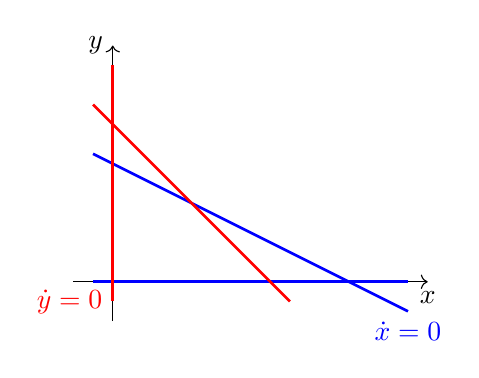
\begin{tikzpicture}
      \draw[->] (-0.5, 0) -- (4, 0) node[below] {$x$};
      \draw[->] (0, -0.5) -- (0, 3) node[left] {$y$};

      \draw[blue, line width=0.333mm] (-0.25, 0) -- (3.75, 0) {};
      \draw[blue, line width=0.333mm, domain=-0.25:3.75] plot (\x, {1.5 - 0.5*\x}) node[below] {$\dot{x} = 0$};

      \draw[red, line width=0.333mm] (0, 2.75) -- (0, -0.25) node[left] {$\dot{y} = 0$};
      \draw[red, line width=0.333mm, domain=-0.25:2.25] plot (\x, {2 - \x}) {};
    \end{tikzpicture}
  \end{minipage}

  \vspace{1cm}
\end{frame}

\begin{frame}[t, c]{Two-dimensional systems}{Example : Rabbits vs.\ Sheeps}
  \begin{minipage}{.48\textwidth}
    At the origin, we have
    %
    \[
    \bm{J} = \begin{bmatrix} 3 & 0 \\ 0 & 2 \end{bmatrix}.
    \]

    The eigenvalues are $\lambda_1 = 3$ and $\lambda_2 = 2$ while the eigenvectors are
    %
    \[
    \bm{v}_1 = \bm{e}_1, \quad \bm{v}_2 = \bm{e}_2.
    \]
    %
    It is an \textbf{unstable node}.
  \end{minipage}%
  \hfill
  \begin{minipage}{.48\textwidth}
    \centering
    \begin{tikzpicture}
      \draw[->] (-0.5, 0) -- (4, 0) node[below] {$x$};
      \draw[->] (0, -0.5) -- (0, 3) node[left] {$y$};

      \draw[->, >=stealth, blue, line width=0.333mm] (0, 0) -- (0.5, 0) {};
      \draw[->, >=stealth, blue, line width=0.333mm] (0, 0) -- (0, 0.5) {};

      \node[circle, fill=white, draw=black, inner sep=0pt, minimum size=4pt] (a) at (0, 0) {};

    \end{tikzpicture}
  \end{minipage}

  \vspace{1cm}
\end{frame}

\begin{frame}[t, c]{Two-dimensional systems}{Example : Rabbits vs.\ Sheeps}
  \begin{minipage}{.48\textwidth}
    At $(x, y) = (3, 0)$, we have
    %
    \[
    \bm{J} = \begin{bmatrix} -3 & -6 \\ 0 & -1 \end{bmatrix}
    \]
    %
    whose eigenvalues are $\lambda_1 = -3$ and $\lambda_2 = -1$.
    This fixed point is thus a \textbf{stable node}.
  \end{minipage}%
  \hfill
  \begin{minipage}{.48\textwidth}
    \centering
    \begin{tikzpicture}
      \draw[->] (-0.5, 0) -- (4, 0) node[below] {$x$};
      \draw[->] (0, -0.5) -- (0, 3) node[left] {$y$};

      \draw[->, >=stealth, blue, line width=0.333mm] (0, 0) -- (0.5, 0) {};
      \draw[->, >=stealth, blue, line width=0.333mm] (0, 0) -- (0, 0.5) {};

      \draw[->, >=stealth, blue, line width=0.333mm] (2.5, 0) -- (3, 0) {};
      \draw[->, >=stealth, blue, line width=0.333mm] (2.525658350974743, 0.15811388300841897) -- (3, 0) {};

      \node[circle, fill=white, draw=black, inner sep=0pt, minimum size=4pt] (a) at (0, 0) {};
      \node[circle, fill=black, draw=black, inner sep=0pt, minimum size=4pt] (a) at (3, 0) {};

    \end{tikzpicture}
  \end{minipage}

  \vspace{1cm}
\end{frame}


\begin{frame}[t, c]{Two-dimensional systems}{Example : Rabbits vs.\ Sheeps}
  \begin{minipage}{.48\textwidth}
    At $(x, y) = (0, 2)$, we have
    %
    \[
    \bm{J} = \begin{bmatrix} -1 & 0 \\ -2 & -2 \end{bmatrix}
    \]
    %
    whose eigenvalues are $\lambda_1 = -2$ and $\lambda_2 = -1$.
    This fixed point is thus a \textbf{stable node}.
  \end{minipage}%
  \hfill
  \begin{minipage}{.48\textwidth}
    \centering
    \begin{tikzpicture}
      \draw[->] (-0.5, 0) -- (4, 0) node[below] {$x$};
      \draw[->] (0, -0.5) -- (0, 3) node[left] {$y$};

      \draw[->, >=stealth, blue, line width=0.333mm] (0, 0) -- (0.5, 0) {};
      \draw[->, >=stealth, blue, line width=0.333mm] (0, 0) -- (0, 0.5) {};

      \draw[->, >=stealth, blue, line width=0.333mm] (2.5, 0) -- (3, 0) {};
      \draw[->, >=stealth, blue, line width=0.333mm] (2.525658350974743, 0.15811388300841897) -- (3, 0) {};

      \draw[->, >=stealth, blue, line width=0.333mm] (0, 1.5) -- (0, 2) {};
      \draw[->, >=stealth, blue, line width=0.333mm] (0.22360679774997896, 1.5527864045000421) -- (0, 2) {};

      \node[circle, fill=white, draw=black, inner sep=0pt, minimum size=4pt] (a) at (0, 0) {};
      \node[circle, fill=black, draw=black, inner sep=0pt, minimum size=4pt] (a) at (3, 0) {};
      \node[circle, fill=black, draw=black, inner sep=0pt, minimum size=4pt] (a) at (0, 2) {};

    \end{tikzpicture}
  \end{minipage}

  \vspace{1cm}
\end{frame}


\begin{frame}[t, c]{Two-dimensional systems}{Example : Rabbits vs.\ Sheeps}
  \begin{minipage}{.48\textwidth}
    At $(x, y) = (1, 1)$, we have
    % 
    \[
    \bm{J} = \begin{bmatrix} -1 & -2 \\ -1 & -1 \end{bmatrix}
    \]
    %
    whose eigenvalues are $\lambda_{1, 2} = -1 \pm \sqrt{2}$.
    This fixed point is thus a \textbf{saddle}.
  \end{minipage}%
  \hfill
  \begin{minipage}{.48\textwidth}
    \centering
    \begin{tikzpicture}
      \draw[->] (-0.5, 0) -- (4, 0) node[below] {$x$};
      \draw[->] (0, -0.5) -- (0, 3) node[left] {$y$};

      \draw[->, >=stealth, blue, line width=0.333mm] (0, 0) -- (0.5, 0) {};
      \draw[->, >=stealth, blue, line width=0.333mm] (0, 0) -- (0, 0.5) {};

      \draw[->, >=stealth, blue, line width=0.333mm] (2.5, 0) -- (3, 0) {};
      \draw[->, >=stealth, blue, line width=0.333mm] (2.525658350974743, 0.15811388300841897) -- (3, 0) {};

      \draw[->, >=stealth, blue, line width=0.333mm] (0, 1.5) -- (0, 2) {};
      \draw[->, >=stealth, blue, line width=0.333mm] (0.22360679774997896, 1.5527864045000421) -- (0, 2) {};

      \draw[<->, >=stealth, blue, line width=0.333mm] (0.591751709536137, 1.2886751345948129) -- (1.4082482904638631, 0.7113248654051871) {};
      \draw[>-<, >=stealth, blue, line width=0.333mm] (0.591751709536137, 0.7113248654051871) -- (1.4082482904638631, 1.2886751345948129) {};

      \node[circle, fill=white, draw=black, inner sep=0pt, minimum size=4pt] (a) at (0, 0) {};
      \node[circle, fill=black, draw=black, inner sep=0pt, minimum size=4pt] (a) at (3, 0) {};
      \node[circle, fill=black, draw=black, inner sep=0pt, minimum size=4pt] (a) at (0, 2) {};
      \node[circle, fill=white, draw=black, inner sep=0pt, minimum size=4pt] (a) at (1, 1) {};

    \end{tikzpicture}
  \end{minipage}

  \vspace{1cm}
\end{frame}


\begin{frame}[t, c]{Two-dimensional systems}{Example : Rabbits vs.\ Sheeps}
  \begin{minipage}{.48\textwidth}
    \begin{overprint}
      \onslide<2>
      \centering
      \begin{tikzpicture}
        \draw[->] (-0.5, 0) -- (4, 0) node[below] {$x$};
        \draw[->] (0, -0.5) -- (0, 3) node[left] {$y$};
        
        \draw[gray, smooth, thick] plot file{traj1.txt};
        \draw[gray, smooth, thick] plot file{traj2.txt};
        \draw[gray, smooth, thick] plot file{traj3.txt};
        \draw[gray, smooth, thick] plot file{traj4.txt};
        \draw[gray, smooth, thick] plot file{traj5.txt};
        \draw[gray, smooth, thick] plot file{traj6.txt};
        \draw[gray, smooth, thick] plot file{traj7.txt};
        \draw[gray, smooth, thick] plot file{traj8.txt};
        
        
        \node[circle, fill=white, draw=black, inner sep=0pt, minimum size=4pt] (a) at (0, 0) {};
        \node[circle, fill=black, draw=black, inner sep=0pt, minimum size=4pt] (a) at (3, 0) {};
        \node[circle, fill=black, draw=black, inner sep=0pt, minimum size=4pt] (a) at (0, 2) {};
        \node[circle, fill=white, draw=black, inner sep=0pt, minimum size=4pt] (a) at (1, 1) {};
        
      \end{tikzpicture}
    \end{overprint}
  \end{minipage}%
  \hfill
  \begin{minipage}{.48\textwidth}
    \centering
    \begin{tikzpicture}
      \draw[->] (-0.5, 0) -- (4, 0) node[below] {$x$};
      \draw[->] (0, -0.5) -- (0, 3) node[left] {$y$};

      \draw[->, >=stealth, blue, line width=0.333mm] (0, 0) -- (0.5, 0) {};
      \draw[->, >=stealth, blue, line width=0.333mm] (0, 0) -- (0, 0.5) {};

      \draw[->, >=stealth, blue, line width=0.333mm] (2.5, 0) -- (3, 0) {};
      \draw[->, >=stealth, blue, line width=0.333mm] (2.525658350974743, 0.15811388300841897) -- (3, 0) {};

      \draw[->, >=stealth, blue, line width=0.333mm] (0, 1.5) -- (0, 2) {};
      \draw[->, >=stealth, blue, line width=0.333mm] (0.22360679774997896, 1.5527864045000421) -- (0, 2) {};

      \draw[<->, >=stealth, blue, line width=0.333mm] (0.591751709536137, 1.2886751345948129) -- (1.4082482904638631, 0.7113248654051871) {};
      \draw[>-<, >=stealth, blue, line width=0.333mm] (0.591751709536137, 0.7113248654051871) -- (1.4082482904638631, 1.2886751345948129) {};

      \node[circle, fill=white, draw=black, inner sep=0pt, minimum size=4pt] (a) at (0, 0) {};
      \node[circle, fill=black, draw=black, inner sep=0pt, minimum size=4pt] (a) at (3, 0) {};
      \node[circle, fill=black, draw=black, inner sep=0pt, minimum size=4pt] (a) at (0, 2) {};
      \node[circle, fill=white, draw=black, inner sep=0pt, minimum size=4pt] (a) at (1, 1) {};

    \end{tikzpicture}
  \end{minipage}

  \vspace{1cm}
\end{frame}

\begin{frame}[t, c]{Two-dimensional systems}{Hartman-Grobman theorem}
  \small
  \begin{minipage}{.58\textwidth}
    \textbf{Theorem :} The behaviour of a dynamical system in a domain near a hyperbolic equilibrium point is qualitatively the same as the behaviour of its linearization near this equilibrium point.

    \bigskip

    A hyperbolic fixed point is a point for which the associated Jacobian matrix has no eigenvalue with zero real part.
  \end{minipage}%
  \hfill
  \begin{minipage}{.38\textwidth}
    \centering
    \includegraphics[width=\textwidth]{fixed_points_classification}
  \end{minipage}

  \vspace{1cm}
\end{frame}

\begin{frame}[t, c]{Two-dimensional systems}{Basins of attraction and separatrices}
  \begin{minipage}{.68\textwidth}
    \small
    Given a fixed point $\bm{x}^*$, its \alert{\textbf{basin of attraction}} is the set of initial conditions $\bm{x}_0$ such that $\bm{x}(t) \to \bm{x}^*$ as $t \to \infty$.

    \bigskip

    The \alert{\textbf{stable manifold}} of the saddle point form the \alert{\textbf{separatrix}} between two different basins.
  \end{minipage}%
  \hfill
  \begin{minipage}{.28\textwidth}
    \centering
    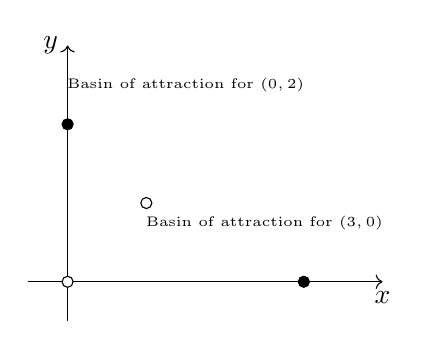
\begin{tikzpicture}
      \draw[->] (-0.5, 0) -- (4, 0) node[below] {$x$};
      \draw[->] (0, -0.5) -- (0, 3) node[left] {$y$};

      \draw[gray, smooth, thick] plot file{traj7.txt};
      \draw[gray, smooth, thick] plot file{traj8.txt};

      \node[] () at (2.5, 0.75) {\tiny Basin of attraction for $(3, 0)$};
      \node[] () at (1.5, 2.5) {\tiny Basin of attraction for $(0, 2)$};


      \node[circle, fill=white, draw=black, inner sep=0pt, minimum size=4pt] (a) at (0, 0) {};
      \node[circle, fill=black, draw=black, inner sep=0pt, minimum size=4pt] (a) at (3, 0) {};
      \node[circle, fill=black, draw=black, inner sep=0pt, minimum size=4pt] (a) at (0, 2) {};
      \node[circle, fill=white, draw=black, inner sep=0pt, minimum size=4pt] (a) at (1, 1) {};

    \end{tikzpicture}
  \end{minipage}

  \vspace{1cm}
\end{frame}

\begin{frame}[t, c]{Two-dimensional systems}{Approximating the stable and unstable manifolds}
  \begin{minipage}{.68\textwidth}
    In the vicinity of $(x^*, y^*) = (1, 1)$, the stable and unstable manifolds can be approximated using a power series expansion.

    \bigskip

    Given the change of variable $\xi = x^* - x$ and $\eta = y^* - y$, our system becomes
    %
    \[
    \begin{aligned}
      \dot{\xi} & = -\xi( 1 + 2\eta +  \xi) - 2\eta\\
      \dot{\eta} & = -\eta (1 + \xi + \eta) - \xi
    \end{aligned}
    \]
    %
    corresponding to a shift of the origin of our phase space to the saddle point $(x^*, y^*) = (1, 1)$.
  \end{minipage}%
  \hfill
  \begin{minipage}{.28\textwidth}
    \centering
    \begin{tikzpicture}
      \draw[->] (-0.5, 0) -- (4, 0) node[below] {$x$};
      \draw[->] (0, -0.5) -- (0, 3) node[left] {$y$};

      \draw[<->, >=stealth, black] (0.591751709536137, 1.2886751345948129) -- (1.4082482904638631, 0.7113248654051871) {};
      \draw[>-<, >=stealth, black] (0.591751709536137, 0.7113248654051871) -- (1.4082482904638631, 1.2886751345948129) {};

      \draw[->, >=stealth, black] (0, 0) -- (0.5, 0) {};
      \draw[->, >=stealth, black] (0, 0) -- (0, 0.5) {};

      \draw[->, >=stealth, black] (2.5, 0) -- (3, 0) {};
      \draw[->, >=stealth, black] (2.525658350974743, 0.15811388300841897) -- (3, 0) {};

      \draw[->, >=stealth, black] (0, 1.5) -- (0, 2) {};
      \draw[->, >=stealth, black] (0.22360679774997896, 1.5527864045000421) -- (0, 2) {};

      \draw[gray, smooth, thick] plot file{traj5.txt};
      \draw[gray, smooth, thick] plot file{traj6.txt};

      \draw[gray, smooth, thick] plot file{traj7.txt};
      \draw[gray, smooth, thick] plot file{traj8.txt};

      \node[circle, fill=white, draw=black, inner sep=0pt, minimum size=4pt] (a) at (0, 0) {};
      \node[circle, fill=black, draw=black, inner sep=0pt, minimum size=4pt] (a) at (3, 0) {};
      \node[circle, fill=black, draw=black, inner sep=0pt, minimum size=4pt] (a) at (0, 2) {};
      \node[circle, fill=white, draw=black, inner sep=0pt, minimum size=4pt] (a) at (1, 1) {};

    \end{tikzpicture}
  \end{minipage}

  \vspace{1cm}
\end{frame}


\begin{frame}[t, c]{Two-dimensional systems}{Approximating the stable and unstable manifolds}
  \begin{minipage}{.68\textwidth}
    In a second step, assume that $\eta = h(\xi)$ so that
    %
    \[
    \dot{\eta} = \dfrac{dh}{d\xi} \dfrac{d\xi}{dt}.
    \]
    %
    Replacing $\eta$ by $h(\xi)$ in our original system yields
    %
    \[
    \underbrace{-h(\xi) \left( 1 + \xi + h(\xi) \right) - \xi}_{\dot{\eta}} = \underbrace{\dfrac{dh}{d\xi} \left( -\xi (1 + 2h(\xi) + \xi) - 2h(\xi) \right)}_{h^{\prime}(\xi) \dot{\xi}}.
    \]
  \end{minipage}%
  \hfill
  \begin{minipage}{.28\textwidth}
    \centering
    \begin{tikzpicture}
      \draw[->] (-0.5, 0) -- (4, 0) node[below] {$x$};
      \draw[->] (0, -0.5) -- (0, 3) node[left] {$y$};

      \draw[<->, >=stealth, black] (0.591751709536137, 1.2886751345948129) -- (1.4082482904638631, 0.7113248654051871) {};
      \draw[>-<, >=stealth, black] (0.591751709536137, 0.7113248654051871) -- (1.4082482904638631, 1.2886751345948129) {};

      \draw[->, >=stealth, black] (0, 0) -- (0.5, 0) {};
      \draw[->, >=stealth, black] (0, 0) -- (0, 0.5) {};

      \draw[->, >=stealth, black] (2.5, 0) -- (3, 0) {};
      \draw[->, >=stealth, black] (2.525658350974743, 0.15811388300841897) -- (3, 0) {};

      \draw[->, >=stealth, black] (0, 1.5) -- (0, 2) {};
      \draw[->, >=stealth, black] (0.22360679774997896, 1.5527864045000421) -- (0, 2) {};

      \draw[gray, smooth, thick] plot file{traj5.txt};
      \draw[gray, smooth, thick] plot file{traj6.txt};

      \draw[gray, smooth, thick] plot file{traj7.txt};
      \draw[gray, smooth, thick] plot file{traj8.txt};

      \node[circle, fill=white, draw=black, inner sep=0pt, minimum size=4pt] (a) at (0, 0) {};
      \node[circle, fill=black, draw=black, inner sep=0pt, minimum size=4pt] (a) at (3, 0) {};
      \node[circle, fill=black, draw=black, inner sep=0pt, minimum size=4pt] (a) at (0, 2) {};
      \node[circle, fill=white, draw=black, inner sep=0pt, minimum size=4pt] (a) at (1, 1) {};

    \end{tikzpicture}
  \end{minipage}

  \vspace{1cm}
\end{frame}


\begin{frame}[t, c]{Two-dimensional systems}{Approximating the stable and unstable manifolds}
  \begin{minipage}{.68\textwidth}
    Assuming that $h(\xi) = a \xi + b \xi^2$, expanding both sides of the equation and regrouping like powers yields the following system for $a$ and $b$
    %
    \[
    \begin{aligned}
      \mathcal{O}(\xi) &: \quad & a^2 = \dfrac{1}{2} \\
      \mathcal{O}(\xi^2) &: \quad & a^2 + (1 + 6a) b = 0.
    \end{aligned}
    \]
    %
    Two sets of solutions exists giving rise to
    %
    \[
    h_{\pm}(\xi) = a_{\pm} \xi + b_{\pm} \xi^2.
    \]
    %
    Here, $h_+(\xi)$ (resp.\ $h_{-}(\xi)$) is the approximation of the stable (resp.\ unstable) manifold.
  \end{minipage}%
  \hfill
  \begin{minipage}{.28\textwidth}
    \centering
    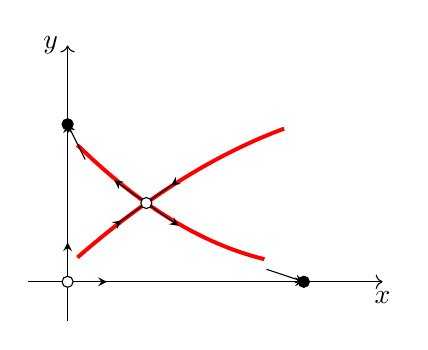
\begin{tikzpicture}
      \draw[->] (-0.5, 0) -- (4, 0) node[below] {$x$};
      \draw[->] (0, -0.5) -- (0, 3) node[left] {$y$};

      \draw[red, line width=0.5mm, domain=0.125:2.75] plot (\x, {1 + (1/sqrt(2))*(\x-1) - 1/(2+6*sqrt(2))*(\x-1)^2}) {};
      \draw[red, line width=0.5mm, domain=0.125:2.5] plot (\x, {1 - (1/sqrt(2))*(\x-1) - 1/(2-6*sqrt(2))*(\x-1)^2}) {};
      \draw[gray, smooth, thick] plot file{traj5.txt};
      \draw[gray, smooth, thick] plot file{traj6.txt};

      \draw[gray, smooth, thick] plot file{traj7.txt};
      \draw[gray, smooth, thick] plot file{traj8.txt};

      \draw[<->, >=stealth, black] (0.591751709536137, 1.2886751345948129) -- (1.4082482904638631, 0.7113248654051871) {};
      \draw[>-<, >=stealth, black] (0.591751709536137, 0.7113248654051871) -- (1.4082482904638631, 1.2886751345948129) {};

      \draw[->, >=stealth, black] (0, 0) -- (0.5, 0) {};
      \draw[->, >=stealth, black] (0, 0) -- (0, 0.5) {};

      \draw[->, >=stealth, black] (2.5, 0) -- (3, 0) {};
      \draw[->, >=stealth, black] (2.525658350974743, 0.15811388300841897) -- (3, 0) {};

      \draw[->, >=stealth, black] (0, 1.5) -- (0, 2) {};
      \draw[->, >=stealth, black] (0.22360679774997896, 1.5527864045000421) -- (0, 2) {};

      \node[circle, fill=white, draw=black, inner sep=0pt, minimum size=4pt] (a) at (0, 0) {};
      \node[circle, fill=black, draw=black, inner sep=0pt, minimum size=4pt] (a) at (3, 0) {};
      \node[circle, fill=black, draw=black, inner sep=0pt, minimum size=4pt] (a) at (0, 2) {};
      \node[circle, fill=white, draw=black, inner sep=0pt, minimum size=4pt] (a) at (1, 1) {};

    \end{tikzpicture}
  \end{minipage}

  \vspace{1cm}
\end{frame}


\begin{frame}[t, c]{Two-dimensional systems}{Oscillatory dynamics}
  \begin{minipage}{.68\textwidth}
    The main interest of two-dimensional systems is their ability to model \alert{\textbf{oscillatory}} behaviours, the canonical example being that of the simple pendulum.

    \bigskip

    Starting from Newton's principles, the equation of motion is given by
    %
    \[
    \ddot{\theta} + \dfrac{g}{L}\sin(\theta) = 0
    \]
    %
    where $\theta$ is the angle of pendulum with respect to the vertical axis.
  \end{minipage}%
  \hfill
  \begin{minipage}{.28\textwidth}
    \centering
    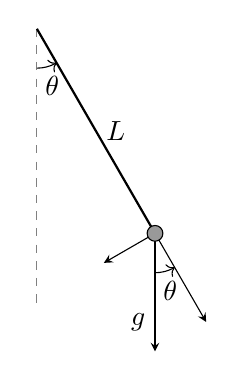
\begin{tikzpicture}
      % save length of g-vector and theta to macros
      \pgfmathsetmacro{\Gvec}{1.5}
      \pgfmathsetmacro{\myAngle}{30}
      % calculate lengths of vector components
      \pgfmathsetmacro{\Gcos}{\Gvec*cos(\myAngle)}
      \pgfmathsetmacro{\Gsin}{\Gvec*sin(\myAngle)}
      
      \coordinate (centro) at (0,0);
      \draw[dashed,gray,-] (centro) -- ++ (0,-3.5) node (mary) [black,below]{$ $};
      \draw[thick] (centro) -- ++(270+\myAngle:3) coordinate (bob) node[midway, right] {$L$};
      \pic [draw, ->, "$\theta$", angle eccentricity=1.5] {angle = mary--centro--bob};
      %\draw [blue,-stealth] (bob) -- ($(bob)!\Gcos cm!(centro)$);
      \draw [-stealth] (bob) -- ($(bob)!-\Gcos cm!(centro)$)
      coordinate (gcos)
      node[midway,above right] {};
      \draw [-stealth] (bob) -- ($(bob)!\Gsin cm!90:(centro)$)
      coordinate (gsin)
      node[midway,above left] {};
      \draw [-stealth] (bob) -- ++(0,-\Gvec)
      coordinate (g)
      node[near end,left] {$g$};
      \pic [draw, ->, "$\theta$", angle eccentricity=1.5] {angle = g--bob--gcos};
      \filldraw [fill=black!40,draw=black] (bob) circle[radius=0.1];
    \end{tikzpicture}
  \end{minipage}

  \vspace{1cm}
\end{frame}

\begin{frame}[t, c]{Two-dimensional systems}{Oscillatory dynamics}
  \begin{minipage}{.58\textwidth}
    Let us consider instead the following system
    %
    \[
    \begin{aligned}
      \dot{x} & = \mu x - y - (x^2 + y^2) x \\
      \dot{y} & = x + \mu y - (x^2 + y^2) y.
    \end{aligned}
    \]
    %
    Its Jacobian matrix reads
    %
    \[
    \bm{J} = \begin{bmatrix} \mu & -1 \\ 1 & \mu \end{bmatrix}
    \]
    and its eigenvalues are $\lambda = \mu \pm i $.
    The origin is thus a stable ($\mu < 0$) or unstable ($\mu > 0$) spiral.
  \end{minipage}%
  \hfill
  \begin{minipage}{.38\textwidth}
    \centering
    \begin{tikzpicture}
      \draw[->] (-2, 0) -- (2, 0) node[below] {$x$};
      \draw[->] (0, -2) -- (0, 2) node[left] {$y$};

      \draw[gray, domain=0:18, smooth, samples=1024, variable=\t, thick] plot ({0.01*exp(0.25*\t) * cos(\t r)}, {0.01*exp(0.25*\t) * sin(\t r)});

      \node[circle, fill=white, draw=black, inner sep=0pt, minimum size=4pt] (a) at (0, 0) {};

    \end{tikzpicture}
  \end{minipage}

  \vspace{1cm}
\end{frame}

\begin{frame}[t, c]{Two-dimensional systems}{Oscillatory dynamics}\
  \begin{minipage}{.32\textwidth}
    \centering
    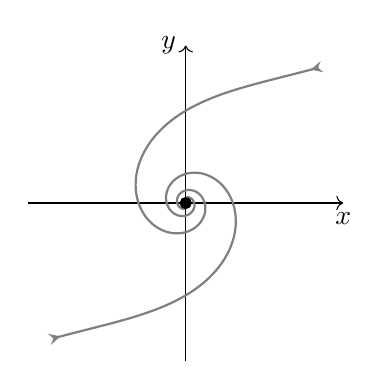
\begin{tikzpicture}
      \draw[->] (-2, 0) -- (2, 0) node[below] {$x$};
      \draw[->] (0, -2) -- (0, 2) node[left] {$y$};

      \draw[>-, >=stealth, gray, domain=0:10, variable=\t, samples=1024, thick] plot ({2*sqrt(-0.25*1.5 / (1.5 + exp(0.5*\t)*(-0.25-1.5))) * cos((\t+pi/4) r)}, {2*sqrt(-0.25*1.5 / (1.5 + exp(0.5*\t)*(-0.25-1.5))) * sin((\t+pi/4) r)});

      \draw[>- , >=stealth, gray, domain=0:10, variable=\t, samples=1024, thick] plot ({2*sqrt(-0.25*1.5 / (1.5 + exp(0.5*\t)*(-0.25-1.5))) * cos((\t-3*pi/4) r)}, {2*sqrt(-0.25*1.5 / (1.5 + exp(0.5*\t)*(-0.25-1.5))) * sin((\t-3*pi/4) r)});

      \node[circle, fill=black, draw=black, inner sep=0pt, minimum size=4pt] (a) at (0, 0) {};

    \end{tikzpicture}

    $$\mu < 0$$
  \end{minipage}
  \hfill
  \begin{minipage}{.32\textwidth}
    \centering
    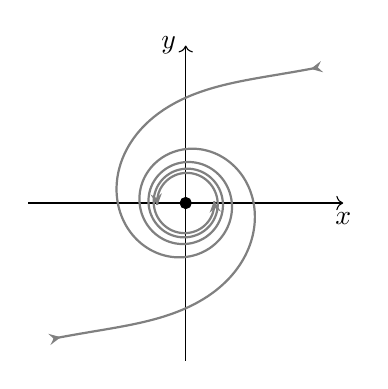
\begin{tikzpicture}
      \draw[->] (-2, 0) -- (2, 0) node[below] {$x$};
      \draw[->] (0, -2) -- (0, 2) node[left] {$y$};


      \draw[>->, >=stealth, gray, domain=0:15, variable=\t, samples=1024, thick] plot ({2*sqrt(1.5/(2*1.5*\t + 1)) * cos((\t+pi/4) r)}, {2*sqrt(1.5/(2*1.5*\t + 1)) * sin((\t+pi/4) r)});

      \draw[>->, >=stealth, gray, domain=0:15, variable=\t, samples=1024, thick] plot ({2*sqrt(1.5/(2*1.5*\t + 1)) * cos((\t-3*pi/4) r)}, {2*sqrt(1.5/(2*1.5*\t + 1)) * sin((\t-3*pi/4) r)});

      \node[circle, fill=black, draw=black, inner sep=0pt, minimum size=4pt] (a) at (0, 0) {};

    \end{tikzpicture}

    $$\mu = 0$$
  \end{minipage}%
  \hfill
  \begin{minipage}{.32\textwidth}
    \centering
    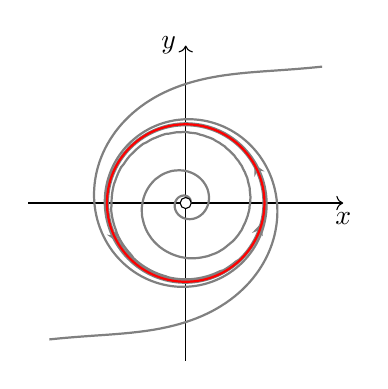
\begin{tikzpicture}
      \draw[->] (-2, 0) -- (2, 0) node[below] {$x$};
      \draw[->] (0, -2) -- (0, 2) node[left] {$y$};

      \draw[->, >=stealth, gray, domain=0:50, variable=\t, samples=1024, thick] plot ({2*sqrt(0.25*0.001 / (0.001 + exp(-0.5*\t)*(0.25-0.001))) * cos(\t r)}, {2*sqrt(0.25*0.001 / (0.001 + exp(-0.5*\t)*(0.25-0.001))) * sin(\t r)});

      \draw[->, >=stealth, gray, domain=0:50, variable=\t, samples=1024, thick] plot ({2*sqrt(0.25*1.5 / (1.5 + exp(-0.5*\t)*(0.25-1.5))) * cos((\t+pi/4) r)}, {2*sqrt(0.25*1.5 / (1.5 + exp(-0.5*\t)*(0.25-1.5))) * sin((\t+pi/4) r)});

      \draw[->, >=stealth, gray, domain=0:50, variable=\t, samples=1024, thick] plot ({2*sqrt(0.25*1.5 / (1.5 + exp(-0.5*\t)*(0.25-1.5))) * cos((\t-3*pi/4) r)}, {2*sqrt(0.25*1.5 / (1.5 + exp(-0.5*\t)*(0.25-1.5))) * sin((\t-3*pi/4) r)});

      \node[circle, fill=white, draw=black, inner sep=0pt, minimum size=4pt] (a) at (0, 0) {};

      \draw[red, thick] (0, 0) circle (1);
    \end{tikzpicture}

    $$\mu > 0$$
  \end{minipage}
  
  \vspace{1cm}
\end{frame}

\begin{frame}[t, c]{Two-dimensional systems}
  \begin{minipage}{.58\textwidth}
    Introducing the complex variable $z = x + i y$, our system can be recast as
    %
    \[
    \dot{z} = (\mu + i)z + \vert z \vert^2 z.
    \]
    %
    Turning to polar coordinates $z = r e^{i\theta}$, the equation becomes
      %
    \[
    \begin{aligned}
      \dot{r} & = \mu r - r^3 \\
      \dot{\theta} & = 1
    \end{aligned}
    \]
      %
    which simplifies the analysis quite a lot.
  \end{minipage}%
  \hfill
  \begin{minipage}{.38\textwidth}
    \begin{overprint}
      \onslide<1>
      \centering
      \begin{tikzpicture}
        \draw[->] (-0.25, 0) -- (2, 0) node[below] {$r$};
        \draw[->] (0, -2) -- (0, 2) node[left] {$\dot{r}$};
        
        \draw[gray, line width=0.5mm, domain=0:1] plot (\x, {-\x - \x^3});
        
        \node[circle, fill=black, draw=black, inner sep=0pt, minimum size=4pt] (a) at (0, 0) {};
        
      \end{tikzpicture}

      $$\mu < 0$$

      \onslide<2>
      \centering
      \begin{tikzpicture}
        \draw[->] (-0.25, 0) -- (2, 0) node[below] {$r$};
        \draw[->] (0, -2) -- (0, 2) node[left] {$\dot{r}$};
        
        \draw[gray, line width=0.5mm, domain=0:2^(1/3)] plot (\x, {- \x^3});
        
        \node[circle, fill=black, draw=black, inner sep=0pt, minimum size=4pt] (a) at (0, 0) {};
        
      \end{tikzpicture}

      $$\mu = 0$$

      \onslide<3>
      \centering
      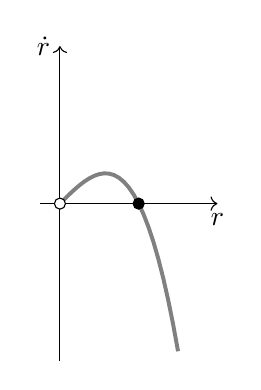
\begin{tikzpicture}
        \draw[->] (-0.25, 0) -- (2, 0) node[below] {$r$};
        \draw[->] (0, -2) -- (0, 2) node[left] {$\dot{r}$};
        
        \draw[gray, line width=0.5mm, domain=0:1.5] plot (\x, {\x - \x^3});
        
        \node[circle, fill=white, draw=black, inner sep=0pt, minimum size=4pt] (a) at (0, 0) {};
        \node[circle, fill=black, draw=black, inner sep=0pt, minimum size=4pt] (a) at (1, 0) {};

      \end{tikzpicture}

      $$\mu > 0$$
    \end{overprint}
  \end{minipage}

  \vspace{1cm}
\end{frame}

\begin{frame}[t, c]{Two-dimensional systems}{Oscillatory dynamics}
  \begin{minipage}{.58\textwidth}
    As $\mu$ becomes positive, the system exhibits periodic dynamics known as a \alert{\textbf{limit cycle}}.

    \bigskip

    For this particular system, this limit cycle is created through a \alert{\textbf{supercritical Hopf bifurcation}} at $\mu = 0$ which will be the subject of an upcoming lecture.
  \end{minipage}%
  \hfill
  \begin{minipage}{.38\textwidth}
    \centering
    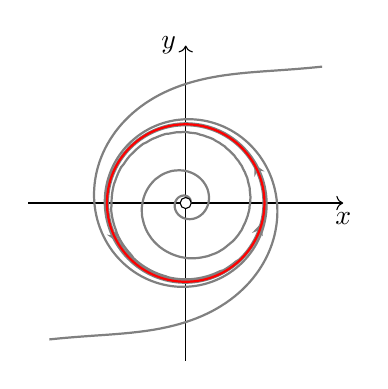
\begin{tikzpicture}
      \draw[->] (-2, 0) -- (2, 0) node[below] {$x$};
      \draw[->] (0, -2) -- (0, 2) node[left] {$y$};

      \draw[->, >=stealth, gray, domain=0:50, variable=\t, samples=1024, thick] plot ({2*sqrt(0.25*0.001 / (0.001 + exp(-0.5*\t)*(0.25-0.001))) * cos(\t r)}, {2*sqrt(0.25*0.001 / (0.001 + exp(-0.5*\t)*(0.25-0.001))) * sin(\t r)});

      \draw[->, >=stealth, gray, domain=0:50, variable=\t, samples=1024, thick] plot ({2*sqrt(0.25*1.5 / (1.5 + exp(-0.5*\t)*(0.25-1.5))) * cos((\t+pi/4) r)}, {2*sqrt(0.25*1.5 / (1.5 + exp(-0.5*\t)*(0.25-1.5))) * sin((\t+pi/4) r)});

      \draw[->, >=stealth, gray, domain=0:50, variable=\t, samples=1024, thick] plot ({2*sqrt(0.25*1.5 / (1.5 + exp(-0.5*\t)*(0.25-1.5))) * cos((\t-3*pi/4) r)}, {2*sqrt(0.25*1.5 / (1.5 + exp(-0.5*\t)*(0.25-1.5))) * sin((\t-3*pi/4) r)});

      \node[circle, fill=white, draw=black, inner sep=0pt, minimum size=4pt] (a) at (0, 0) {};

      \draw[red, thick] (0, 0) circle (1);

    \end{tikzpicture}
  \end{minipage}

  \vspace{1cm}
\end{frame}

\end{document}
